% This is an AMS-LaTeX v. 1.2 File.

\documentclass{report}

%\usepackage{showkeys}
\usepackage[T2A]{fontenc}
\usepackage[utf8]{inputenc}
\usepackage[english,russian]{babel}
\usepackage{expdlist}
\usepackage{graphicx}
\usepackage{amsmath}
\usepackage{amssymb}
\usepackage{amsthm}
\usepackage{amsfonts}
\usepackage{amsxtra} 
\usepackage{sty/dbl12}
\usepackage{srcltx}
\usepackage{epsfig}
\usepackage{verbatim}
\usepackage{sty/rac}
\usepackage{listings}


%%%%%%%%%%%%%%%%%%%%%%%%%%%%%%%%%%%%%%%%%%%%%%%%%%%%%%%%%%%%%%%%%%%%%%%%%%%%%%

% Redefine margins and other page formatting

\setlength{\oddsidemargin}{0.5in}

\theoremstyle{plain}                                                                                                                                                                
\newtheorem{theorem}{Теорема}                                                                                                                         
\newtheorem{prop}[theorem]{Утверждение}
                                                                                                                                                                                      
\theoremstyle{definition}                                                                                                                                                             
\newtheorem{definition}[theorem]{Определение}                                                                                                                                         

%%%%%%%%%%%%%%%%%%%%%%%%%%%%%%%%%%%%%%%%%%%%%%%%%%%%%%%%%%%%%%%%%%%%%%%%%%%%%%%

\numberwithin{theorem}{chapter}

\binoppenalty=10000
\relpenalty=10000

\graphicspath{{pic/}}

\begin{document}


\bibliographystyle{alpha}

\initializefrontsections
\pagestyle{title}

\begin{center}
Санкт-Петербургский государственный университет \\ информационных технологий, механики и оптики

\vspace{2cm}

Кафедра компьютерных технологий

\vspace{3cm}

{\Large А. А. Давыдов}

\vspace{2cm}

\vbox{\LARGE\bfseries
Применение методов спектральной теории графов для внедрения цифровых водяных знаков в двумерные векторные данные}
\vspace{4cm}

Дипломная работа 

\vspace{1cm}

{\Large Научный руководитель --- к.ф.-м.н., доцент С. Ю. Жуков}

\vspace{5cm}

Санкт-Петербург\\ 2011
\end{center}


\newpage

\setcounter{page}{3}
\pagestyle{plain}

\tableofcontents

% Chapters

\startprefacepage

Цифровые водяные знаки (ЦВЗ) --- технология созданная для защиты авторских прав мультимедийных файлов,
однако в настоящее время этот термин принято понимать в более широком смысле, а именно, как технологию
внедрения некоторой информации в цифровые данные. В частности, в данной работе нас будет интересовать
внедрение ЦВЗ в данные географических информационных систме (ГИС).

ГИС оперируют геометрическими примитивами (точки, полилинии, контура), с аттрибутами 
произвольного типа. В общем случае для внедрения можно использовать только геометрические данные,
то есть задача создания ЦВЗ для ГИС-данных является частным случаем задачи создания ЦВЗ для двумерных векторных данных.

Жизненный цикл ЦВЗ состоит из следующих фаз.
\begin{itemize}
  \item Модификация исходных данных (внедрение водяных знаков) для добавления к данным 
  некоторого сообщения, скажем, фамилии автора или названия компании-владельца. 
  На этом этапе может применяется секретный ключ. 
  \item Атаки модифицированных данных злоумышленником, то есть изменения их с целью уничтожения 
  или изменения водяных знаков.
  \item Извлечение водяных знаков из атакованных данных, для доказательства авторских прав.
\end{itemize}

Основными требованиями, предъявляемыми к алгоритмам внедрения ЦВЗ являются:
\begin{enumerate}
  \item устойчивость к атакам --- способность извлекать внедренные ЦВЗ из атакованных данных;
  \item незначительность искажения исходных данных при внедрении.
\end{enumerate}

Очевидно, что эти требования конфликтуют, и обычно при разработке алгоритма внедрения ЦВЗ
больше внимания уделяется первому из них. Цель данной работы --- разработка критерия степени искажения
ГИС-данных и разработка устойчивого к атакам алгоритма внедрения ЦВЗ
минимизирующего предложенный критерий.



\startthechapters

\chapter{Базовый алгоритм}

В данной главе приводится формальная постановка задачи (\ref{sec:prob_def}), 
краткая классификация алгоритмов внедрения (\ref{sec:classification}) и затем
излагаеися краткое описание алгоритма предложеннго в работе \cite{Ohbuchi}, в дальнейшем называемого базовым~ 
(\ref{sec:base}), и приводится неформальное обоснование корректности его работы~(\ref{sec:explanation}).
\section{Формальная постановка задачи}
\label{sec:prob_def}

ГИС-данные --- это планарный прямолинейный граф $G = (V, E)$, обладающий следующими свойствами:
\begin{itemize}
    \item кластеризованность;
    \item равномерное распределение вершин внутри кластера.
\end{itemize}
Кроме того для ГИС-данных характерен масштаб и допустимая погрешность.

В дальнейшем вместо термина ``граф'' будет часто употребляться термин ``карта''. Будем также использовать термин 
\textit{оригинальная} для исходной карты, термин \textit{подписанная} для карты с внедренными 
ЦВЗ и термин \textit{атакованная} для подписанной карты подвергшейся атаке злоумышленника.

Подписанная карта может подвергаться следубщим видам атак.
\begin{description}
    \item[Переупорядочивание.] Возможное переупорядочивание данных злоумышленником исключает возможнсть 
    использования порядка на вершинах или ребрах графа для внедрения ЦВЗ.
    \item[Преобразование подобия.] Злоумышленник может к применить движения плоскости или 
    равномерное масштабирование множества точек карты без какого-либо ущерба для визуального качества. 
    \item[Вставка и удаление вершин.] Это возможно при упрощении или наоборот сглаживании конутров и полилиний. 
    Очевидно, алгоритм внедрения ЦВЗ, способный противостоять данной атаке, не может рассчитывать даже на то, что количество вершин в исходной и атакованной карты совпадает.
    \item[Шум.] Применение аддитивного случайного шума к координатам вершин. Некоторые авторы \cite{Kim, Shao, Bazin} считают, 
    что требования предъявляемые к точности карт используемых в ГИС столь высоки, что они не позволяют злоумышленникам использовать данный вид атак,
    соответственно, разработанные данными авторами алгоритмы неустойчивы к нему.
    \item[Обрезка (cropping).] Это самая ``сильная'' атака, только один из известных автору алгоритм (\cite{Ohbuchi}) частично устойчив к ней.
\end{description}  

Очевидно, что алгоритмы, устойчивые к хотя бы первым трем из перечисленных видов атак, должные изменять координаты вершин графа, 
но при этом нет смысла добавлять/удалять вершины, или менять их порядок. 
Кроме того существует важное требование, предъявляемое алгоритмам внедрения ЦВЗ --- сохранение топологии графа, из которого, в частности следует,
что множество ребер не должно изменяться.
Таким образом, задача решаемая в данной работе формулируется следующим образом. 
\begin{itemize}
    \item Защитить авторские права на ГИС-данные, изменяя координаты вершин в пределах допустимой погрешности. 
    Изменение координат вершин не должно нарушать топологии графа.
    \item Сформулировать критерий $K$ степени искажения исходных данных.
\end{itemize}
Или более формально.
\begin{itemize}
    \item Найти функцию $f(V_G, key, msg) \to V_G'$, такую что существует обратная функция $\exists f^{-1}(g(V_G'), V_G, key) \to msg$, где
    \begin{itemize}
        \item $key$ --- секретный ключ;
        \item $msg$ --- внедряемое сообщение, удостоверяющее авторство;
        \item $g: V_G' \to V_G''$ --- атака злоумышленником.
    \end{itemize}
    \item Определить и минимизировать функцию $K(G, V_G') \to \mathbb{R}$.
\end{itemize}

\section{Классификация алгоритмов внедрения ЦВЗ}
\label{sec:classification}
Все алгоритмы внедрения ЦВЗ в двумерные векторные данные можно, грубо говоря, поделить на две категории: 
работающие в ``пространственной'' области, и работающие в ``частотной'' области. 
Алгоритмы, принадлежащие первой категории, изменяюют непосредственно 
координаты вершин \cite{Kim, Chang, Bazin}. Алгоритмы из второй категории вычисляют некоторые 
взаимно-однозначно связанные с координатами вершин коэффициенты (дискретное преобразование Фурье, 
дискретное косинусное преобразование, дискретные вейвлет-преобразования и т.д.), изменяют их, а затем 
преобразуют обратно в уже измененные координаты \cite{Voight, Ohbuchi, Ohbuchi3D, Praun}.  
Сильной стороной алгоритмов, принадлежащих первой категории, является возможность контролировать искажение
исходных данных при внедрении ЦВЗ, однако алгоритмы из второй категории более устойчивы к атакам.
Для сохранения топологии графа алгоритмами, работающими в частотной области, можно применить довольно естественную идею,
предлагаемую в работе \cite{Huber}, а именно, ограничить 
возможные смещения вершин областями, определяемыми обобщенной диаграммой Вороного (\cite{Held}), что, очевидно,
гаранитирует отсутствие пересечений в подписанной карте. 
Другим преимуществом алгоритмов, работающих в частотной области, считается их устойчивость к преобразованиям
подобия, так как частотные коэффициенты сохраняются.
Однако это существенно только если при атаке карты не используется вставка/удаление вершин или 
при вычислении частотных коэффициентов число вершин не важно (пример такого алгоритма в работе \cite{Shao}). 

Другим признаком, по которому можно классифицировать алгоритмы внедрения, является использование 
оригинальной карты для извлечения ЦВЗ. Те алгоритмы, которые требуют оригинальной карты для извлечения ЦВЗ,
называются хорошо информированными (well-informed), в противоположность им не требующие, называются ослепленными
(blinded). Ослепленность есть весьма полезное свойство в случае больших карт, производимых на лету, 
так как она избавляет от необходимости хранить оригинальные версии, однако, очевидно, она уменьшает возможности
извлечения, а значит, и внедрения ЦВЗ.

\section{Алгоритм Обучи}
\label{sec:base}

Лучшим в смысле устойчивости к атакам из известных автору алгоритмов является алгоритм предложенный 
Ohbuchi et al. в работе \cite{Ohbuchi}. Это хорошо информированный, работающий в частотной области алгоритм,
главная идея которого заключается в применении техники, разработанной для трехмерной полигональной сетки к
двумерным картам.
Для вычисления частотного представления планарного графа строится его триагуляция Делоне с ограничениями 
(\cite{Chew}), и для получившейся сетки вычисляется частотное представление, используя спектральный анализ 
предложенный в работах \cite{Karni1, Karni2}. Затем частотные коэффициенты изменяются согласно битам 
внедряемого сообщения. Обратным преобразованием модифицированных коэффициентов в координаты вершин получается
карта с внедренными водяными знаками. Изменение коэффициенто в частотной области влечет смещение вершин в 
пространственной области.

Для увеличения эффективности вычислений и устойчивости против обрезки карта вначале делится на прямоугольные 
области содержащие примерно одинаковое количество вершин (рис. \ref{pic_ohbuchi}). 
\begin{figure}
  \centering
  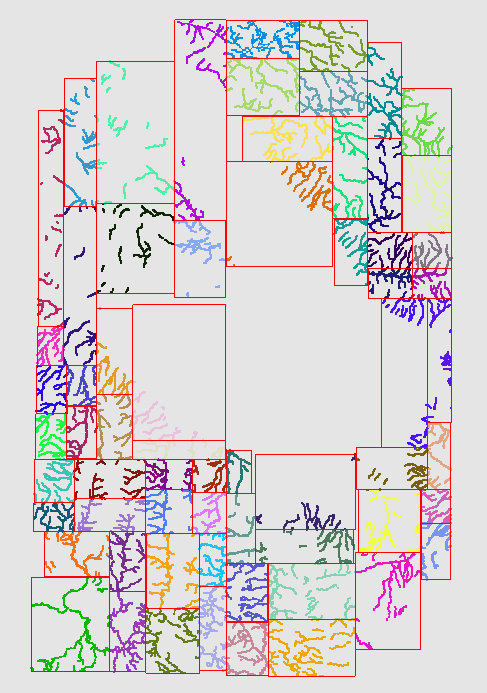
\includegraphics[scale=1.0]{ohbuchi.png}
  \caption{Разбиение карты на области}
  \label{pic_ohbuchi}
\end{figure}
Упомянутые выше спектральный анализ и внедрения водяных знаков производится для каждой области независимо.

Водяные знаки извлекаются сранением орининальной и атакованной карты. В первую очередь карты геометрически
''регистрируются'' с помощью итеративного процесса минимизации расстояния между множествами предварительно
выбранных пометок. Эта регистрация может устранить аффинное преобразование примененное к подписанной карте.

Для вставки вершин удаленных злоумышленником и удаления вершин вставленных злоумышленников используется 
следующий алгоритм. Для каждой вершины оригинальной
карты осуществляется поиск вершин в круге некоторого радиуса на атакованной карте. Если не было найдено ни одной,
вершины то соответсвующая вершина добавляется, если было найдено несколько, то удаляются все кроме ближайшей
к соответствующей вершине оригинальной карты.

Рассмотрим процесс внедрения ЦВЗ подробнее.  
Пусть $V = \{v_1, v_2, \dots, v_n\}$ есть множество вершин оригинальной карты, $n = |V|$. 
Пусть $\mathfrak{T}$ озбозначает некоторую триангуляцию множества $V$, $G(\mathfrak{T})$ обозначает 
граф триангуляции $\mathfrak{T}$. Собственные вектора $\{\mathbf{e}_i\}_{i=1}^n$ графа $G(\mathfrak{T})$ суть 
собственные вектора его лапласиана. 
Существует несколько определений лапласиана графа, к примему \cite{Biggs, Chung, Zhang}. В базовом алгоритме 
используется определение данное в \cite{Biggs}
$$R = I - D^{-1} A,$$ где $I$ --- единичная матрицв, $D$ --- диагональная матрица составленная из 
степеней вершин графа $G(\mathfrak{T})$, $A$ --- матрица смежности $G(\mathfrak{T})$
\begin{eqnarray*}
  D_{ij} = \begin{cases} deg(v_i) &\text{if $i = j$,} \\ 0 &\text{otherwise;} \end{cases} \\
  A_{ij} = \begin{cases} 1 &\text{if vertices $i$ and $j$ is adjacent,} \\ 0 &\text{otherwise.} \end{cases} 
\end{eqnarray*}
Собственные вектора $\{\mathbf{e}_i\}_{i=1}^n$ составляют базис $\mathbb{R}^n$. Будем предполагать, что 
собственные вектора нормализованны, $||e_i|| = 1$. 
Пусть $v_i = (x_i, y_i)$ тогда $\mathbf{r} = (r_1, r_2, \dots, r_n)$, $\mathbf{s} = (s_1, s_2, \dots, s_n)$ 
суть разложения векторов $\mathbf{x} = (x_1, x_2, \dots, x_n)^T$, $\mathbf{y} = (y_1, y_2, \dots, y_n)^T$ 
соответственно в базисе $\{\mathbf{e}_i\}_{i=1}^n$. Другими словами 
\begin{eqnarray*}
  \mathbf{x} = r_1 \mathbf{e}_1 + r_2 \mathbf{e}_2 + \dots + r_n \mathbf{e_n}; \\ 
  \mathbf{y} = s_1 \mathbf{e}_1 + s_2 \mathbf{e}_2 + \dots + s_n \mathbf{e_n}.  
\end{eqnarray*}
Если $\{\mathbf{e}_i\}_{i=1}^n$ ортогональны, то $r_i = (\mathbf{x}, \mathbf{e}_i)$, 
$s_i~=~(\mathbf{y}, \mathbf{e}_i)$, но в общем случае это не верно. 

Предположим, что внедряемое сообщение $\mathbf{m} = (m_1, m_2, \dots, m_k)$ состоит из $k$ бит, где $k \le n$, 
$m_i \in \{0, 1\}$. Введем обозначение $q_i = 2 * m_i - 1$, $q_i \in \{-1, 1\}$.
Изменим коэффициенты $r_i, s_i$, $1 \le k \le n$ следующим образом
\begin{eqnarray*}
  r_i' = r_i + \alpha p_i q_i; \\
  s_i' = s_i + \alpha p_i q_i, 
\end{eqnarray*}
где $\{p_i\}$ есть псевдослучайная последовательность, $\alpha$ --- некоторая положительная константа. 
Увеличение ~$\alpha$ увеличивает устойчивость к атакам на внедренные ЦВЗ, но вызывает большее искажение
карты. 

Пусть $\mathbf{x'}, \mathbf{y'}$ координаты вершин подписанной карты. 
\begin{eqnarray*}
  \mathbf{x'} - \mathbf{x} = (r_1' - r_1) \mathbf{e}_1 + (r_2' - r_2) \mathbf{e}_2 + \dots + (r_n' - r_n) \mathbf{e_n} = \\
  = \alpha \left[ p_1 q_1 \mathbf{e}_1 + p_2 q_2 \mathbf{e}_2 + \dots + p_k q_k \mathbf{e}_k \right], \\
  \mathbf{y'} - \mathbf{y} = \alpha \left[ p_1 q_1 \mathbf{e}_1 + p_2 q_2 \mathbf{e}_2 + \dots + p_k q_k \mathbf{e}_k \right]. 
\end{eqnarray*}
Другими словами внедрение ЦВЗ может быть выражено как построение вектора  
\begin{equation}
\label{formula:g}
 \mathbf{g} = \alpha \left[ p_1 \mathbf{h}_1 + p_2 \mathbf{h}_2 + \dots + p_k \mathbf{h}_k \right]; 
\end{equation}
$$ \mathbf{h_i} = \left( \begin{pmatrix} e_{i, 1} \\ e_{i, 1} \end{pmatrix} 
\begin{pmatrix} e_{i, 2} \\ e_{i, 2} \end{pmatrix}, \dots, \begin{pmatrix} e_{i, n} \\e_{i, n}  \end{pmatrix} 
\right), 1 \le i \le n. $$
Если вектора $\{\mathbf{e}_i\}_{i=1}^n$ ортонормированны, можно оценить среднее по всем вершинам расстояние 
смещения $\Delta v_{mean}$.
\begin{equation}
\label{formula:mean_displacement}
|\mathbf{g}| = \alpha * \sqrt {k} * \sqrt{2}; \mbox{      } \Delta v_{mean} = \alpha * \frac{\sqrt{2k}}{n}. 
\end{equation}

Для извлечение водяных знаков необходимо разложить вектора $\mathbf{x'} - \mathbf{x}$, 
$\mathbf{y'} - \mathbf{y}$ в базисе $\{\mathbf{e}_i\}_{i=1}^k$, то есть вычислить коэффициенты 
$\mathbf{u} = (u_1, u_2, \dots, u_k)$, $\mathbf{w} = (w_1, w_2, \dots, w_k)$, 
\begin{eqnarray*}
  \mathbf{x'} - \mathbf{x} = u_1 \mathbf{e}_1 + u_2 \mathbf{e}_2 + \dots + u_k \mathbf{e_k}; \\ 
  \mathbf{y'} - \mathbf{y} = w_1 \mathbf{e}_1 + w_2 \mathbf{e}_2 + \dots + w_k \mathbf{e_k}.  
\end{eqnarray*}
Биты внедренного сообщения получаются так:
$$q_i = \sgn(p_i * (u_i + w_i)), m_i = (q_i + 1) / 2.$$

\section{Обоснование корректности}
\label{sec:explanation}
Будем считать, что единственный вид атак, которым подвергается подписанная карта --- аддитивный случайный шум, примененный к координатам вершин, 
так как сопоставление множества вершин оригинальной и атакованной карты, применяемое в процедуре извлечения ЦВЗ базового алгоритма 
(\ref{sec:base}), позволяет свести все другие атаки также к добавлению к координатам вершин 
небольшой случайной (с точки зрения злоумышленника) величины.

Рассмотрим простейшую модель. Пусть действительное число $x$, чтобы закодировать бит $b = \pm 1$, преобразуется в $x' = x + b \alpha$, 
где $\alpha$~---~некоторая константа. Затем $x'$ атакуется случайным шумом c амплитудой $\sigma$, то есть преобразуется в $x'' = x' + y$,
где $y$ --- случайная величина с функцией распределения $F(t) = \Phi(t / \sigma)$, $\Phi$ --- функция Лапласа. Для извлечения бита вычисляется
$b' = \sgn(x'' - x)$. Вероятность того, что бит будет правильно извлечен, равна 
$
P[\sgn(x'' - x) = b] = P[\sgn(b \alpha + n) = b] = F(\alpha) = \Phi(\alpha / \sigma).
$

Чуть усложним модель. Пусть теперь для кодирования одного бита $b$ используется набор $\left\{x_j\right\}_{j=1}^n$
из $n=2k+1$ вещественных чисел, каждое из которых преобразуется также как в предыдущей модели,
для извлечения бита вычисляется $\sgn\left(\sum_{j=1}^n b_j'\right)$. Вероятность того, что бит будет извлечен правильно, равна 
$P\left(\left|\{j | b_j' = b, j = 1..n\}\right| \ge k + 1\right) = \sum_{j=0}^k \binom{n}{j} p^{n-j}(1-p)^j$, где $p = \Phi(\alpha / \sigma)$.
Если ввести обозначение $q = 1 - p$, $P_n = \sum_{j=0}^k \binom{n}{j} p^{n-j} q^j$, то будет верно следующее утверждение:
\begin{equation}
\label{prob_rec}
P_n = P_{n-2} + \binom{n-2}{k-1} p^k q^k (p - q),
\end{equation}
откуда видно, что для увеличения надежности кодирования бита можно увеличивать как $\alpha$, так и $n$. 
\begin{proof}
\begin{multline*}
\textstyle P_n = \binom{n}{0} p^{n} + \binom{n}{1} p^{n-1} q + \binom{n}{2} p^{n-2} q^2 + \ldots + \binom{n}{k-1} p^{k+2} q^{k-1} + \binom{n}{k} p^{k+1} q^k = \\
\shoveleft \textstyle = \left[\binom{n-1}{0} p^n + \binom{n-1}{0} p^{n-1} q \right] + \left[\binom{n-1}{1} p^{n-1} q + \binom{n-1}{1} p^{n-2} q^2 \right]
+ \ldots \\
\shoveright{\textstyle + \left[\binom{n-1}{k-1}p^{k+2}q^{k-1} + \binom{n-1}{k-1}p^{k+1}q^k \right] + \binom{n-1}{k}p^{k+1}q^k =} \\
\shoveleft \textstyle = \binom{n-1}{0} p^{n-1} + \binom{n-1}{1}p^{n-2}q + \ldots + \binom{n-1}{k-1}p^{k+1}q^{k-1} + \binom{n-1}{k} p^{k+1} q^k = \\
\shoveleft \textstyle = \left[\binom{n-2}{0}p^{n-1} + \binom{n-2}{0} p^{n-2} q \right] + \left[\binom{n-2}{0}p^{n-1} + \binom{n-2}{0} p^{n-2} q \right] +
\ldots \\
\shoveright{\textstyle + \left[\binom{n-2}{k-2}p^{k+2}q^{k-2} + \binom{n-2}{k-2}p^{k+1}q^{k-1} \right] + 
\binom{n-2}{k-1}p^{k+1}q^{k-1} + \binom{n-1}{k}p^{k+1}q^{k} = }\\
\shoveleft \textstyle = \left[\binom{n-2}{0} p^{n-2} + \binom{n-2}{1}p^{n-3}q + \ldots + \binom{n-2}{k-2}p^{k+1}q^{k-2} \right] + 
\binom{n-2}{k-1}p^{k+1}q^{k-1} + \binom{n-1}{k}p^{k+1}q^{k} = \\
\shoveleft \textstyle = P_{n-2} - \binom{n-2}{k-1}p^{k}q^{k-1} + \binom{n-2}{k-1}p^{k+1}q^{k-1} + \binom{n-1}{k}p^{k+1}q^{k} = \\ 
\shoveleft \textstyle = P_{n-2} + \binom{n-2}{k-1} p^{k}q^{k-1} (p - 1) + \left(\binom{n-2}{k-1} + \binom{n-2}{k} \right) p^{k+1}q^{k} = \\
\textstyle = P_{n-2} - \binom{n-2}{k-1} p^{k}q^{k} + 2p \binom{n-2}{k-1} p^k q^k = P_{n-2} + \binom{n-2}{k-1} p^k q^k (p - q). 
\end{multline*}
\end{proof}

Таким образом, для кодирования внедрения сообщения, состоящего из $m$ бит, можно было бы просто изменить координаты $m * n$ вершин карты на величину равную по модулю $\alpha$, где
$n$ и $\alpha$ выбираются из расчета того, какой амплитуды случайному шуму должны противостоять водяные знаки. Почему же все-таки выгоднее работать в частотной области?

Во-первых, длина внедряемого сообщения, как правило, много меньше числа вершин карты, а значит, чтобы изменение координат было равномерно 
по всем вершинам, надо выбирать достаточно большое $n$. В то же время из формулы~(\ref{prob_rec}) видно, что с ростом $n$ вероятность 
правильного извлечения сообщения растет довольно медленно, а значит с точки зрения устойчивости к атакам при одинаковом 
суммарном изменении координат вершин было бы выгодно брать небольшое значение $n$ и большое значение~$\alpha$.

Во-вторых, отметим, что переход от естественного базиса $\mathbb{R}^d$ к собственным векторам лапласиана, это есть в точности преобразование Фурье. 
А преобразование Фурье обладает принципом неопределенности, то есть, грубо говоря, невозможно произвольно сконцентрировать и функцию и ее Фурье-образ.
В частности для дискретного преобразования Фурье (ДПФ) в работе~\cite{Uncertainty} этот принцип сформулирован следующим образом. 
Пусть $\{\mathbf{j}\}_{j=0}^{d-1}$, $\{\tilde{\mathbf{k}}\}_{k=0}^{d-1}$ --- два ортонормированных базиса $\mathbb{C}^d$ связанных ДПФ:
\begin{equation*}
\textstyle |\tilde{\mathbf{k}} \rangle = \sum\limits_{j=0}^{d-1} \frac{e^{i 2\pi j k / d}}{\sqrt{d}} |\mathbf{j} \rangle,\mbox{    }
|{\mathbf{j}} \rangle = \sum\limits_{k=0}^{d-1} \frac{e^{i 2\pi j k / d}}{\sqrt{d}} |\tilde{\mathbf{k}} \rangle.
\end{equation*}
Если рассмотреть унитарные операторы 
$$
U = \sum\limits_{j=0}^{d-1} e^{i 2\pi j / d} |\mathbf{j} \rangle \langle \mathbf{j} |,\mbox{    }
U = \sum\limits_{k=0}^{d-1} e^{i 2\pi k / d} |\tilde{\mathbf{k}} \rangle \langle \tilde{\mathbf{k}} |,
$$
то их дисперсии
$$
\textstyle
\Delta U^2 = 1 - |\langle \psi | U | \psi \rangle |^2, \mbox{   }
\Delta V^2 = 1 - |\langle \psi | V | \psi \rangle |^2, \mbox{   } |\psi|^2 = 1,
$$
будут связаны соотношением $\Delta U^2 \Delta V^2 \ge \frac{\pi^2}{d^2}$ или $\Delta U^2 = (0|1), \Delta V^2 = (1|0)$. Отсюда в частности следует, что если вектор $\psi$ имеет координаты 
$\left(\frac{1}{\sqrt{d}}, \frac{1}{\sqrt{d}}, \ldots, \frac{1}{\sqrt{d}}\right)$ в одном базисе, он равен какому-то базисному вектору другого базиса.
В случае преобразования используемого в базовом алгоритме (и его модификации предложенной в данной работе) это тоже выполняется. Действительно, константный вектор на вершинах графа 
является его собственным вектором соответсвующим собственному числу $0$.

Считая, что вектор шума состоит из случайных величин с мат. ожиданием $0$ и одинаковой дисперсией, независимо заданных для каждой вершины графа, можно утверждать, 
что после преобразования Фурье они сконцентрируются около нескольких частот, а значит, большинство внедренных битов будет правильно извлечено с высокой вероятностью.


\chapter{Оценка искажения}

Существует два аспекта искажения исходных данных при внедрении ЦВЗ. Это, во-первых, нарушение топологии графа,
то есть возникновения пересечений между отрезками подписанной карты не только по концам. Во-вторых, искажение
карты определяется ухудшением ее визуального качества.

Первому аспекту посвящена работа \cite{Huber}. В ней предлагается довольно естественная идея ограничить 
возможные смещения вершин областями определяемыми обобщенной диаграммой Вороного (\cite{Held}), что, очевидно,
гаранитирует отсутствие пересечений в подписанной карте.

Визуальное качество карты понятие плохо формализованное. Попытке все-таки оценить его численно посвящена данная
глава. Очевидно, преобразования подобия не искажают карту, а преобразования подобия это все те преобразования, 
которые сохраняют углы при вершинах геометрических 
примитивов, составляющих карту. Поэтому естественно предположить, что искажение карты определяется изменениями
углов между смежными ребрами исходного графа.

Оригинальная и подписанная карты могут быть рассмотрены как связные области на плоскости, поэтому можно сначала
изложить предлагаемые идеи в непрерывном случае (\ref{sec:continious}), а затем вернуться к 
дискретному~(\ref{sec:discrete}). Затем будет показано~(\ref{sec:minimization}), как модифицировать 
базовый алгоритм~(\ref{sec:base}), для минимизации предлагаемой в данной главе меры искажения.

\section{Непрерывный случай}
\label{sec:continious}

\section{Дискретный случай}
\label{sec:discrete}

Рассмотрим множества sets $V = \left\{v_1, v_2, ... , v_n\right\}, 
V' = \left\{v_1', v_2', ... , v_n'\right\}$, $v_i, v_i' \in \mathbb{R}^2$, $|V| = |V'| = n$. 
Пусть функция $f: V \to V'$ отображает множество $V$ на множество $V'$, $f(v_i) = v_i'$, $1 \le i \le n$. 
Пусть $\Omega$ обозначает выпуклую оболочку $V$. 
Можно построить кусочно-линейную интерполяционную поверхность (КЛИП) значений функции 
$\left\{f(v_i)\right\}_{i=1}^n$ используя какую-либо триангуляцию $\mathfrak{T}$ множества $V$, 
таким образом можно смотреть на $f$ как на функцию бьющую из $\Omega$ в $\mathbb{R}^2$. 
Если точка $v$ лежит в треугольнике $\triangle T = (v_i v_j v_k)$, $\triangle T \in \mathfrak{T}$; $
v = \alpha v_i + \beta v_j + \gamma v_k$, $0 \le \alpha, \beta, \gamma \le 1$, $\alpha + \beta + \gamma = 1$, 
то $f(v) = \alpha f(v_i) + \beta f(v_j) + \gamma f(v_k)$.

Известным фактом (\cite{Pinkall93}) является, что если $f$ --- КЛИП значений 
$\left\{f_i = f(v_i)\right\}_{i=1}^n$ по триангуляции $\mathfrak{T}$, то
\begin{equation*}
  E_D(f) = \frac{1}{4} \sum_{\triangle (i, j, k) \in \mathfrak{T}} \cot{\alpha_{ij}}|f_i - f_j|^2 
  + \cot{\alpha_{jk}}|f_j - f_k|^2 + \cot{\alpha_{ki}}|f_k - f_i|^2,
\end{equation*}
где $\alpha_{ij}$ --- угол противоположный ребру $(v_i, v_j)$ в треугольнике $\triangle T = (v_i, v_j, v_k)$.   

Однако в работе \cite{Pinkall93} заявляется, что очевидно, что верен куда более общий факт, но доказательства не
приводится. Докажем его для одного треугольника $T = \triangle ABC$ и функции $f: T \to \mathbb{R}$ линейной
на нем. Заметим, что это практически то, что нам и требуется, так как $E_D(f) = E_D(f_x) + E_D(f_y)$. 

Пусть $A=(x_1, y_1), B=(x_2, y_2), C=(x_3, y_3)$; $$E_D(f) = \int_{T}{||\nabla{f}||^2 dT} = 
        \int_{T}{\left[\left(\frac{\partial f}{\partial x}\right)^2 + 
                       \left(\frac{\partial f}{\partial y}\right)^2 \right] dx dy}.$$ 

Перейдем к барицентрическим координатам $u, v$: $$T = \left\{(u, v)\mbox{ } | \mbox{ } (u, v) \in \left[0, 1 \right]^2 ,\mbox{ } u + v <= 1 \right\}.$$ 
Введя обозначения \begin{multline*} \Delta = (x_1 - x_3) (y_2 - y_3) - (x_2 - x_3) (y_2 - y_3), \\ \Delta_u = (y_2 - y_3) x - (x_2 - x_3) y, \mbox{ } \Delta_v = -(y_1 - y_3) x + (x_1 - x_3) y, 
\end{multline*}
Легко вывести
\begin{multline*} u = \frac{\Delta_u}{\Delta}, \mbox{ } v = \frac{\Delta_v}{\Delta} \mbox{, } dxdy = |\Delta| dudv; \\
        \frac{\partial u}{\partial x} = \frac{1}{\Delta}(y_2 - y_3), \mbox{ } \frac{\partial u}{\partial y} = -\frac{1}{\Delta}(x_2 - x_3) \mbox{; }
        \frac{\partial v}{\partial x} = -\frac{1}{\Delta}(y_1 - y_3), \mbox{ } \frac{\partial v}{\partial y} = \frac{1}{\Delta}(x_1 - x_3); \\
        f(u, v) = f_1 u + f_2 v + f_3(1-u-v) = (f_1 - f_3) u + (f_2 - f_3) v; \\
        \frac{\partial f}{\partial u} = f_1 - f_3 \mbox{, } \frac{\partial f}{\partial v} = f_2 - f_3. 
\end{multline*} 
 \begin{multline*}
        \frac{\partial f}{\partial x} = \frac{\partial f}{\partial u} \frac{\partial u}{\partial x} + \frac{\partial f}{\partial v} \frac{\partial v}{\partial x} = 
            \frac{1}{\Delta}(y_2 - y_3)(f_1 - f_3) - \frac{1}{\Delta}(y_1 - y_3)(f_2 - f_3) = \\
            \frac{1}{\Delta}\left[(y_2 - y_3)(f_1 - f_3) - (y_1 - y_3)(f_2 - f_3)\right]. 
    \end{multline*}
    \begin{multline*}
        \frac{\partial f}{\partial y} = \frac{\partial f}{\partial u} \frac{\partial u}{\partial y} + \frac{\partial f}{\partial v} \frac{\partial v}{\partial y} = 
            -\frac{1}{\Delta}(x_2 - y_3)(f_1 - f_3) + \frac{1}{\Delta}(x_1 - x_3)(f_2 - f_3) = \\
            \frac{1}{\Delta}\left[-(x_2 - x_3)(f_1 - f_3) + (x_1 - x_3)(f_2 - f_3)\right]. 
    \end{multline*}
    \begin{multline*}
        \left[\left(\frac{\partial f}{\partial x}\right)^2 + \left(\frac{\partial f}{\partial y}\right)^2 \right] = 
        \frac{1}{\Delta^2} 
        [
            (f_1 - f_3)^2 [(y_2 - y_3)^2 + (x_2 - x_3)^2] + \\ + (f_2 - f_3)^2 [(y_1 - y_3)^2 + (x_1 - x_3)^2] % - \\
            - 2 (f_1 - f_3)(f_2 - f_3)((y_2 - y_3)(y_1 - y_3) + (x_2 - x_3)(x_1 - x_3))
        ].
    \end{multline*}
    Введем обозначения: $\vect{AB} = \vect{c}$, $\vect{BC} = \vect{a}$, $\vect{CA} = \vect{b}$. Тогда предыдущую формулу можно записать следующим образом.
    \begin{multline*}
        \left[\left(\frac{\partial f}{\partial x}\right)^2 + \left(\frac{\partial f}{\partial y}\right)^2 \right] = 
        \frac{1}{\Delta^2} 
        \left[
            (f_1 - f_3)^2 a^2 + (f_2 - f_3)^2 b^2 - 2 (f_1 - f_3)(f_2 - f_3)(\vec{a}, \vec{b}) 
        \right] = \\
        = \frac{1}{\Delta^2} 
        \left[
            (f_1 - f_3)^2 a^2 + (f_2 - f_3)^2 b^2 - (f_1 - f_3)(f_2 - f_3)(a^2 + b^2 - c^2) 
        \right] = \\
        = \frac{1}{\Delta^2} 
        \left[
            a^2 (f_1 - f_3)^2 + b^2 (f_2 - f_3)^2 - (a^2 + b^2 - c^2)(f_1 f_2 - f_3(f_1 + f_2) + f_3^2)
        \right] = \\
        = \frac{1}{2 \Delta^2} 
        [
            2 a^2 (f_1 - f_3)^2 + 2 b^2 (f_2 - f_3)^2 - (a^2 + b^2 - c^2) \times \\
            \times ([2 f_1 f_2 - f_1^2 - f_2 ^ 2] + [f_1 ^2 - 2 f_3 f_1 + f_3 ^ 2] + [f_2^2 - 2 f_3 f_2 + f_3^2])
        ] = \\
      \end{multline*}
      \begin{multline*}
        = \frac{1}{2 \Delta^2} 
        [
            2 a^2 (f_1 - f_3)^2 + 2 b^2 (f_2 - f_3)^2 - 
            \left( a^2 + b^2 - c^2 \right) \times \\ \times \left(-(f_1 - f_2)^2 + (f_1 - f_3)^2 + (f_2 - f_3)^2 \right)
        ] = \\
        = \frac{1}{2 \Delta^2} 
        \left[
            (a^2 + b^2 - c^2)(f_1 - f_2)^2 + (a^2 + c^2 - b^2)(f_1 - f_3)^2 + (b^2 + c^2 - a^2)(f_2 - f_3)^2 
        \right] = \\
        = \frac{1}{\Delta^2} 
        \left[
            ab \cos{(\gamma)} (f_1 - f_2)^2 + ac \cos{(\beta)}(f_1 - f_3)^2 + bc \cos{(\alpha)}(f_2 - f_3)^2 
        \right] = \\
        = \frac{2S(T)}{\Delta^2} 
        \left[
            \cot{(\gamma)} (f_1 - f_2)^2 + \cot{(\beta)}(f_1 - f_3)^2 + \cot{(\alpha)}(f_2 - f_3)^2 
        \right].
    \end{multline*}
    \begin{multline*}
        \int_{T}{\left[\left(\frac{\partial f}{\partial x}\right)^2 + \left(\frac{\partial f}{\partial y}\right)^2 \right] dx dy} = \\
        = \int\limits_0^1\int\limits_0^{1-u} \frac{2S(T)}{\Delta^2} 
        \left[
            \cot{(\gamma)} (f_1 - f_2)^2 + \cot{(\beta)}(f_1 - f_3)^2 + \cot{(\alpha)}(f_2 - f_3)^2 
        \right] 
        |\Delta| du dv = \\
        = \frac{2S(T)}{|\Delta|} 
        \left[
            \cot{(\gamma)} (f_1 - f_2)^2 + \cot{(\beta)}(f_1 - f_3)^2 + \cot{(\alpha)}(f_2 - f_3)^2 
        \right]
        \int\limits_0^1\int\limits_0^{1-u} du dv = \\ 
        = \frac{S(T)}{|\Delta|} 
        \left[
            \cot{(\gamma)} (f_1 - f_2)^2 + \cot{(\beta)}(f_1 - f_3)^2 + \cot{(\alpha)}(f_2 - f_3)^2 
        \right].
    \end{multline*}
    Осталось заметить, что $|\Delta| = 2S(T)$. Окончательно получаем 
    $$
        \int_T ||\nabla{f}||^2 dT = \frac{1}{2} \left[ \cot{(\gamma)} (f_1 - f_2)^2 + \cot{(\beta)}(f_1 - f_3)^2 + \cot{(\alpha)}(f_2 - f_3)^2 \right] 
    $$
\begin{equation}
\label{formula:Pinkall}
  E_D(f) = \frac{1}{4} \sum_{T \in \mathfrak{T}} \left[ \cot{(\gamma)} (f_1 - f_2)^2 + \cot{(\beta)}(f_1 - f_3)^2 + \cot{(\alpha)}(f_2 - f_3)^2 \right].
\end{equation}

Формула~(\ref{formula:Pinkall}) может быть записана как 
\begin{equation}
\label{formula:EDOverEdges}
  E_D(f) = \frac{1}{4} \sum_{\left( i, j \right) \in E\left(\mathfrak{T}\right)}{w_{ij} |f_i - f_j|^2}, 
\end{equation}
где $E(\mathfrak{T})$ есть множество ребер триангуляции $\mathfrak{T}$, 
$w_{ij}~=~\cot\alpha_{ij}~+~\cot\alpha_{ji}$, $\alpha_{\left\{{ij, ji}\right\}}$~---~углы 
противолежащие ребру~$v_i v_j$ в смежных треугольках $\triangle T_1=v_i v_j v_{k_1}$, 
$\triangle T_2~=~v_j v_i v_{k_2}$. Если ребро~$v_i v_j$ принадлежит тольно одному треугольнику 
$v_i v_j v_k$ ($v_i v_j$ принадлежит границе $\Omega$), то $w_{ij} = \cot \alpha_{ij}$.
Если мы предположим, что $f$ --- комплексно-значная функция, то есть  
$$f_x=\re{f}=\frac{1}{2}\left(f + \conjugate{f}\right), f_y=\im{f}=\frac{1}{2}\left(f - \conjugate{f}\right),$$ 
то $$|f_i - f_j|^2 = \conjugate{(f_i - f_j)}(f_i - f_j) = (\conjugate{f_i} - \conjugate{f_j})(f_i - f_j).$$ 

Пусть $G(\mathfrak{T})$ обозначает взвешенный граф триангуляции $\mathfrak{T}$, $V(G) = V$, $E(G) = E(\mathfrak{T})$, вес ребра $(u, v) = w_{uv}$. 
Если рассмотреть лапласиан $L$ графа $G$ определенный следующим образом (\cite{Chen}) 
$$ L_{uv} = \begin{cases}
  \sum_{(v, x) \in E(G)}{w_{vx}}&\text{if $u = v,$} \\
  -w_{uv}&\text{if $u \sim v,$} \\
  0 &\text{otherwise;}
\end{cases}
$$ то формула~(\ref{formula:EDOverEdges}) будет эквивалентна следующей:
\begin{equation}
  \label{formula:EDOverLaplacian}
  E_D(f) = \frac{1}{4} \conjugate{\mathbf{f}^T} L \mathbf{f},
\end{equation}
где $\mathbf{f} = (f_1, f_2, \dots f_n)^T$, $\conjugate{\mathbf{f}^T} = 
(\conjugate{f_1}, \conjugate{f_2}, \dots, \conjugate{f_n})$. Заметим, что $L$ --- вещественный и 
симметричный, а значит, эрмитов.

$\int_{\Omega} \det(\nabla f) d\Omega$ также может быть выражен как некоторая 
эрмитова квадратичная форма, примененная к $\mathbf{f}$. 
Рассмотрим треугольник $\triangle T = v_i v_j v_k \in \mathfrak{T}$. 
$f$ линейна на $\triangle T$, следовательно $\det (\nabla f)$ есть константа, 
а следовательно, $\int_{\triangle T} \det (\nabla f) dT$ есть ориентированная площадь 
$\triangle T' = f_i f_j f_k$. 
Если предположить, что $v_i, v_j, v_k$ образуют левый поворот,~то
\begin{multline}
  \label{formula:det}
  \int_{\triangle T} \det (\nabla f) dT = \frac{1}{2} (f_i - f_k) \times (f_j - f_k) = \\
  = \frac{1}{2} \left[(f_i - f_k)_x (f_j - f_k)_y - (f_i - f_k)_y (f_j - f_k)_y \right] = \\
  = \frac{i}{4} \left[ (f_i - f_k)\conjugate{(f_j - f_k)} - (f_j - f_k) \conjugate{(f_i - f_k)} \right] = \\
  = \frac{i}{4} \left[ (f_i \conjugate{f_j} - \conjugate{f_i} f_j) + (f_j \conjugate{f_k} - \conjugate{f_j} f_k) + 
    (f_k \conjugate{f_i} - \conjugate{f_k} f_i) \right].  
\end{multline}
Подставляя (\ref{formula:det}) в формулу
\begin{equation}
  \label{formula:det_global}
  \int_{\Omega} \det {\left( \nabla f \right) } d\Omega = \sum_{\triangle T \in \mathfrak{T}}{ \int_{\triangle T} \det{ \left(\nabla f \right) } dT},
\end{equation}
можно заметить, что для каждого ребра $v_i v_j$ лежащего внутри выпуклой оболочки $\Omega$  
существует парное ребро $v_j v_i$, а следовательно, выражение 
$(f_i \conjugate{f_j}~-~\conjugate{f_i} f_j)$ содержится в правой части равенства (\ref{formula:det_global}) 
вместе с противоположным выражением $(f_j \conjugate{f_i}~-~\conjugate{f_j} f_i)$, то есть аннигилирует. 
Следовательно, формула (\ref{formula:det_global}) может быть переписана следующим образом
\begin{equation}
\label{formula:det_over_edges}
  \int_{\Omega} \det {\left( \nabla f \right) } d\Omega = \frac{i}{4} \sum_{v_i v_j \in \partial E}{(f_i \conjugate{f_j} - \conjugate{f_i} f_j)},
\end{equation}
где $\partial E = \partial \Omega \cap E(\mathfrak{T})$ --- множество ребер 
триангуляции $\mathfrak{T}$ принадлежащих границе $\Omega$. 
Если рассмотреть эрмитову матрицу $L'$ определенную следующим образом
\begin{equation*}
  L_{uv}' = \begin{cases}
    i  & \text{if edge $uv \in \partial E$ and $\Omega$ is left of the line $(u, v)$;} \\ 
    -i & \text{if edge $uv \in \partial E$ and $\Omega$ is right of the line $(u, v)$;} \\ 
    0  & \text{otherwise}
  \end{cases}
\end{equation*}
то формула~(\ref{formula:det_over_edges}) будет эквивалента следующией:
\begin{equation}
\label{formula:DetOverLaplacian}
  \int_{\Omega} \det {\left( \nabla f \right) } d\Omega = \frac{1}{4} \conjugate{\mathbf{f}^T} L' \mathbf{f}.
\end{equation}
Пользуясь формулами (\ref{formula:EC}), (\ref{formula:EDOverLaplacian}), 
(\ref{formula:DetOverLaplacian}) можно выразить $E_C(f)$ как значение некоторой квадратичной 
формы, примененной к $\mathbf{f}$
\begin{equation*}
  E_C(f) = \frac{1}{4}\conjugate{\mathbf{f}^T} L'' \mathbf{f},
\end{equation*}
где $L'' = L - L'$. Легко видеть, что оператор $L''$ --- эрмитов (как разность двух эрмитовых), 
следовательно, его собственные числа вещественны и из его из его собственных векторов можно составить 
ортонормированный базис~$\mathbb{C}^n$.

\section{Модификация базового алгоритма}
\label{sec:minimization}

Если $\mathbf{f} = \alpha \left[ p_1 \mathbf{e}_1 + p_2 \mathbf{e}_2 + \dots + p_k \mathbf{e}_k \right],$ 
где $\alpha$ --- некоторая положительная константа, $p_i \in \left\{-1, 1 \right\}$ и 
$\{\mathbf{e}_i\}_{i=1}^k$ --- ортонормированная система веторов, то 
$E_C(f) = \frac{1}{4}\conjugate{\mathbf{f}^T} L'' \mathbf{f}$ будет минимизировано, 
когда $\{\mathbf{e}_i\}_{i=1}^k$ суть собственные вектора $L''$ соответствующии $k$ наименьшим 
собственным числам. 

Базовый алгоритм (\ref{sec:base}) строил вектор $\mathbf{g}$ разниц между новыми и старыми
координатми вершин (формула (\ref{formula:g})), а $E_C$ --- функционал применяемый к $f$, 
$f(v) = v + g(v)$. Здесь нет противоречия, так как $$E_C(g) = E_C(f - v) = E_C(f),$$ ибо
функционал $E_C$ линейный и тождественная функция $id(v) = v$ конформна. 

Таким образом, чтобы минимизировать конформную энергию при использовании базового алгоритма 
необходимо выбрать вектора $\{\mathbf{h}_i\}_{i=1}^k$ из формулы (\ref{formula:g}) равными собстенным векторам $L''$, соответсвующим наименьшим собственным числам.

Конформная энергия была определена (\ref{sec:continious}) как мера искажения локальных углов.
Можно посмотреть, что выражает $E_C(f)$ в терминах углов триангуляции $\mathfrak{T}$. 
\begin{multline*}
  E_C(f) = E_D(f) - \int_{\Omega} \det (\nabla f) d\Omega = \\ 
  = \frac{1}{4} \sum_{v_i v_j v_k \in \mathfrak{T}} \cot{\alpha_{ij}}|f_i - f_j|^2 + 
  \cot{\alpha_{jk}}|f_j - f_k|^2 + \cot{\alpha_{ki}}|f_k - f_i|^2 - 4S(f_i f_j f_k),
\end{multline*}
где $S(f_i f_j f_k)$ есть ориентированная площать треугольника $\triangle f_i f_j f_k$. 
В предположении, что функция $f$ не сильно искажает область $\Omega$, 
ориентация треугольника $\triangle f_i f_j f_k$ равна ориентации треугольника 
$\triangle v_i v_j v_k$, то есть треугольник $\triangle f_i f_j f_k$ ориентирован против часовой
стрелки,
\begin{multline*}
  4 S(f_i f_j f_k) = \cot{\alpha_{ij}'}|f_i - f_j|^2 + \cot{\alpha_{jk}'}|f_j - f_k|^2 + \cot{\alpha_{ki}'}|f_k - f_i|^2,
\end{multline*}
где $\alpha_{ij}'$, $\alpha_{jk}'$, $\alpha_{ki}'$ --- углы, противолежащие сторонам $f_i f_j$, 
$f_j f_k$, $f_k f_i$ треугольника $\triangle f_i f_j f_k$ соответственно. 
Таким образом, при определенных предположениях
\begin{multline*}
  E_C(f) = \frac{1}{4} \sum_{v_i v_j v_k \in \mathfrak{T}} (\cot{\alpha_{ij}} - \cot{\alpha_{ij}'})|f_i - f_j|^2 + \\
  + (\cot{\alpha_{jk}} - \cot{\alpha_{jk}'})|f_j - f_k|^2 + (\cot{\alpha_{ki}} - \cot{\alpha_{ki}'})|f_k - f_i|^2,
\end{multline*} откуда видно, что подобные треугольники перешедшие при внедрении ЦВЗ в подобные,
дают вклад в меру искажения пропорциональный своей площади, что довольно естественно.

До этого момента на триангуляцию $\mathfrak{T}$ не накладывалось никаких условий, но очевидно, что
$E_C$ depends on $\mathfrak{T}$. Во-первых, было доказано, что минимизация $E_C$ влечет 
минимизацию углов триангуляции в целом, но наиболее важны с точки зрения визуального качества
карты угла между смежными ребрами исходных контуров и полилиний. Поэтому логично, 
добавить исходные контура и полилинии в триангуляцию $\mathfrak{T}$ как ограничения.
Во-вторых, при переходе от дискретного к непрерывному случаю триангуляция была использована для
построения кусочно-линейной интерполяционной поверхности, поэтому она должна быть выбрана так,
чтобы минимизировать погрешность интерполяции. Согласно теореме Rippa (\cite{Rippa}), 
триангуляция Делоне доставляет наименьшую погрешность КЛИП среди всех триангуляций 
множества точек.
Но так как для доказательства теоремы Rippa необходим только локальный критерий 
пустого круга(\cite{Chen}), она легко обобщается и на случай триангуляций с ограничениями

Таким образом, при построении сетки для вычисления частотного представления карты в 
базовом алгоритме (\ref{sec:base}) действительно имеет смысл строить триангуляцию Делоне 
с ограничениями. 


\chapter{Экспериментальные результаты}
\begin{figure}[h]
  \centerline {
    \mbox{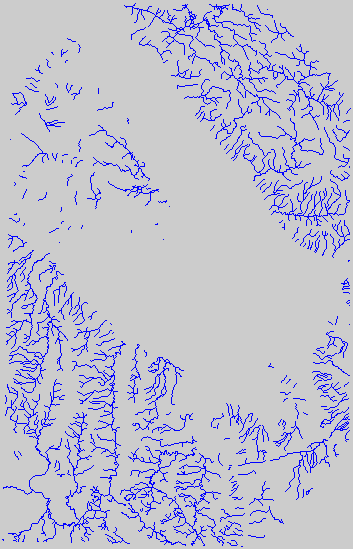
\includegraphics[height=6cm]{rr.png}}
    \mbox{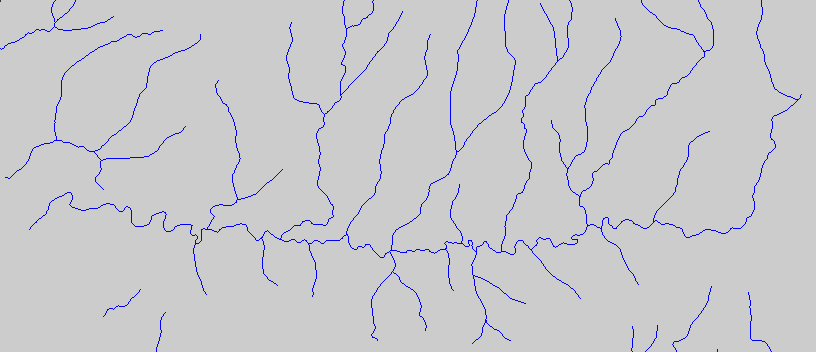
\includegraphics[height=6cm]{rr-small.png}}
  }
  \caption{Рыбинск, реки}
  \label{pic:input_maps}
\end{figure}
\begin{figure}[h]
  \centerline {
    \mbox{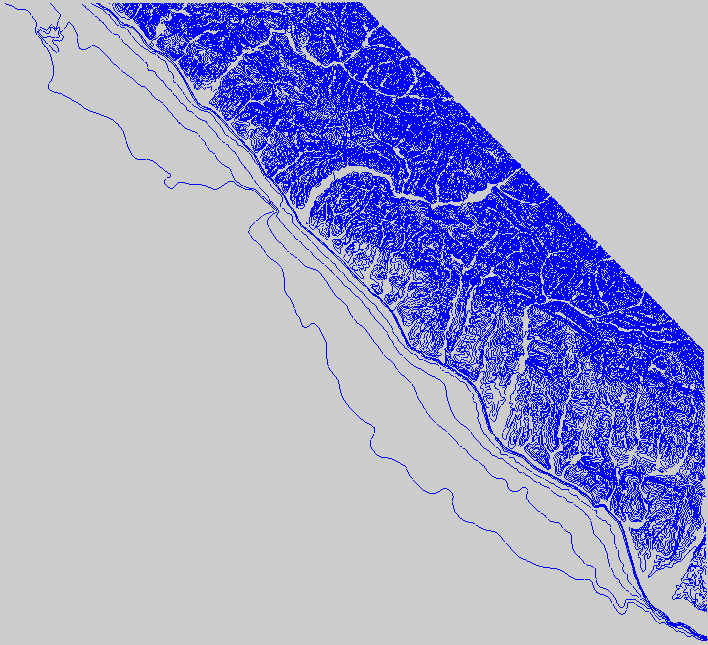
\includegraphics[height=6cm]{si.png}}
    \mbox{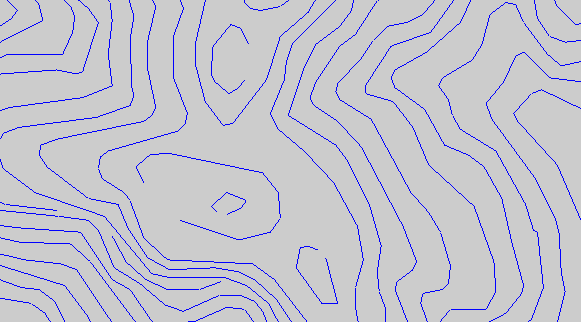
\includegraphics[height=6cm]{si-small.png}}
  }
  \caption{Сочи, изолинии высот}
  \label{pic:input_maps}
\end{figure}



\newpage

\startconclusionpage


\bibliography{thesis}

\end{document}
